\documentclass[tikz, border=5mm]{standalone}
\usepackage{amsmath, amssymb}
\usetikzlibrary{arrows.meta, calc, decorations.markings, shadows}

% Define custom colors for the concepts
\definecolor{volumeColor}{HTML}{FFEDCC} % Pale orange for interior
\definecolor{boundaryColor}{HTML}{CCE5FF} % Pale blue for surface
\definecolor{omegaColor}{HTML}{0066CC}    % Dark blue for boundary form omega
\definecolor{domegaColor}{HTML}{FF6600}   % Dark orange for interior form d_omega

\begin{document}
	
	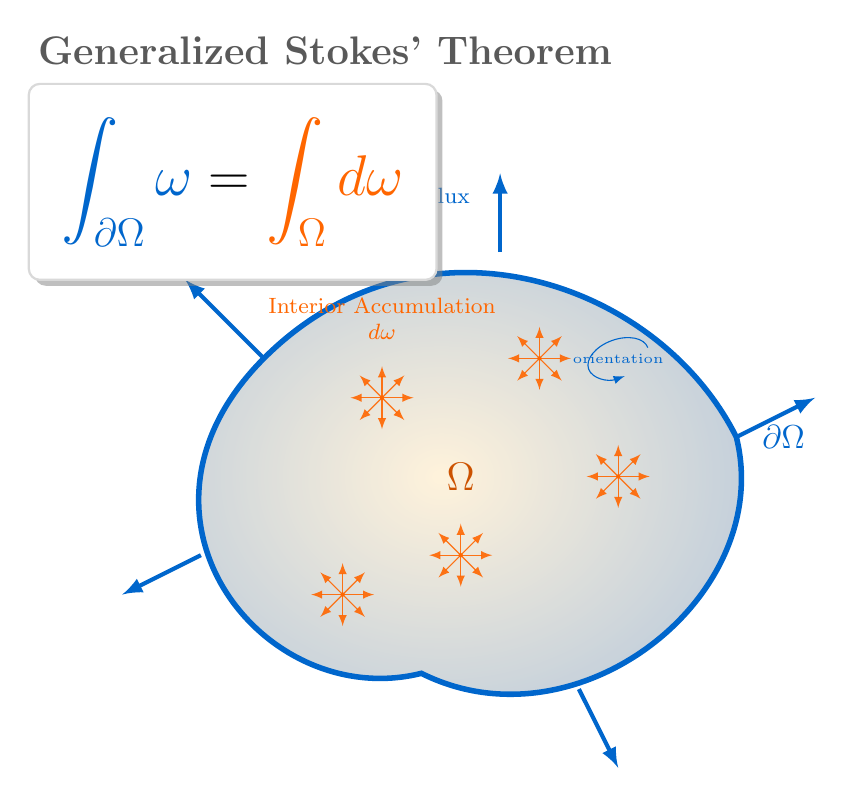
\begin{tikzpicture}[font=\sffamily, >=latex, thick]
		
		% --- 1. Define shape path ---
		% A generic, smooth 3D-looking blob
		\def\blobPath{
			(0, 1) 
			.. controls (2, 3) and (5, 2) .. (6, 0) 
			.. controls (6.5, -2) and (4, -4) .. (2, -3) 
			.. controls (0, -3.5) and (-2, -1) .. (0, 1)
		}
		
		% --- 2. Fill the Interior Volume (Omega) ---
		% Use shading to give depth
		\shade[inner color=volumeColor, outer color=boundaryColor!80!black, opacity=0.7] \blobPath;
		
		% --- 3. Visualize the Interior Form (d_omega) ---
		% Represented as small "sources" or "micro-curls" expanding inside
		\begin{scope}
			\clip \blobPath; % Keep them inside the shape
			\foreach \x/\y in {1.5/0.5, 3.5/1, 2.5/-1.5, 4.5/-0.5, 1/-2} {
				\begin{scope}[shift={(\x,\y)}, scale=0.4, domegaColor, opacity=0.9]
					\foreach \angle in {0, 45, ..., 315} {
						\draw[->, thin] (0,0) -- (\angle:1);
					}
					\fill (0,0) circle (2pt);
				\end{scope}
			}
		\end{scope}
		
		% --- 4. Draw the Boundary Surface (partial Omega) ---
		\draw[omegaColor, line width=2pt] \blobPath;
		
		% --- 5. Visualize the Boundary Form (omega) and Orientation ---
		% Represented as vectors piercing the surface outwards
		
		% Helper to draw boundary vectors based on visual normal approximation
		\foreach \px/\py/\nx/\ny in {
			0/1/-1/1,      % Top left
			3/2.35/0/1,    % Top middlepeak
			6/0/1/0.5,     % Right
			4/-3.2/0.5/-1, % Bottom right
			-0.8/-1.5/-1/-0.5 % Bottom left
		} {
			\draw[->, omegaColor, line width=1.5pt] (\px, \py) -- ++(\nx, \ny);
		}
		
		% Add an orientation swirl on the surface
		\begin{scope}[shift={(4.5, 1)}, rotate=20, scale=0.8]
			\draw[->, omegaColor, thin] (0.5,0) arc (0:270:0.5 and 0.3);
			\node[omegaColor, font=\tiny] at (0,0) {orientation};
		\end{scope}
		
		
		% --- 6. Labels ---
		% Label Omega (Interior)
		\node[domegaColor!80!black, font=\Large] at (2.5, -0.5) {$\Omega$};
		
		% Label Boundary Omega
		\node[omegaColor, font=\large, anchor=west] at (6.2, 0) {$\partial\Omega$};
		
		% Label the concepts visually
		\node[domegaColor, align=center, font=\footnotesize] at (1.5, 1.5) {Interior Accumulation\\$d\omega$};
		\node[omegaColor, align=center, font=\footnotesize, anchor=south west] at (0.5, 2.5) {Boundary Flux\\$\omega$};
		
		
		% --- 7. The Main Formula Box ---
		\node[
		anchor=north west, 
		fill=white, 
		draw=gray!30, 
		rounded corners, 
		drop shadow, 
		inner sep=12pt,
		font=\huge
		] at (-3, 4.5) {
			$\displaystyle 
			\color{omegaColor} \int_{\partial\Omega}\omega
			\color{black} =
			\color{domegaColor} \int_{\Omega} d\omega$
		};
		
		% Add title
		\node[anchor=south west, font=\bfseries\Large, gray!70!black] at (-3, 4.6) { Generalized Stokes' Theorem};
		
	\end{tikzpicture}
	
\end{document}